\chapter{Die Operationen \label{ch:funk}}

...

\section{Die Operatoren $E$ und $U$ \label{sec:eu} }
%\section{Die $E \: \Phi \: U \: \Psi $ - Operation \label{sss:eu} }
\subsubsection*{Die $E \: \Phi \: U \: \Psi $ - Operation \label{sss:eu} }

Die Operationen dienen dem Model-Checking als eine Pr�finstanz der Eigenschaften und der Spezifikation. Dazu werden der Schaltung mittels der Operatoren sinnbildlich Fragen gestellt, deren Antworten die Richtigkeit einer Eigenschaft/Bedingung widergeben. 
Die f�r die $E \: \Phi \: U \: \Psi $ - Operation formulierte Frage w�rde wie folgt aussehen:
%(Ab�ndern)In Worten l�sst sich die $E \: \Phi \: U \: \Psi $ - Operation wie folgt ausgedr�ckt:
\begin{description}
  \item[] Auf welchen Pfaden gilt $\Phi$, bis unmittelbar danach $\Psi$ gilt?
\end{description}
%Es gilt immer $\Psi$ bis $\Phi$ gilt. Es existiert kein Pfad, auf dem $\neg\Phi$ gilt bis $\neg\Psi$ und $\neg\Phi$ gelten und es existiert kein Pfad, auf dem $\Phi$ nie g�ltig wird.
Im \textbf{zeitunbeschr�nkten} Fall, werden durch $E \: \Phi \: U \: \Psi $ die Zust�nde in die Ergebnismenge eingef�gt, die auf einem Pfad in $\Phi$ liegen, welcher unmittelbar nach $\Phi$ in $\Psi$ landet. F�r die gefundenen Zust�nde gilt somit, dass auf mindestens einem Pfad $\Psi$ unmittelbar auf $\Phi$ folgt.
Eine \textbf{Zeitbeschr�nkung} erschwert die Erf�llbarkeit von $E \: \Phi \: U \: \Psi $. Der Operator $E \: \Phi \: U \left[ t_{low}, t_{high} \right] \: \Psi $ restriktiert die Erf�llung auf ein Zeitintervall. Nur Zust�nde von Pfaden, die innerhalb von $\left[ t_{low}, t_{high} \right]$ von $\Phi$ unmittelbar nach $\Psi$ kommen, werden zur Ergebnismenge hinzugef�gt.
Daraus l�sst sich ableiten, dass folgende Teilmengenrelation zu gelten hat: 
\begin{equation}
  E \: \Phi \: U \left[ t_{low}, t_{high} \right] \: \Psi \ \subseteq  E \: \Phi \: U \: \Psi .	\notag
\end{equation}
Abbildung \ref{fig:eu_z} zeigt einen Zustandsgraphen und die jeweilige Ergebnismenge, die aus der Fallunterscheidung \glq keine und eine zeitlichen Begrenzung\grq{} resultiert. Die gr�n markierten Knoten stellen die Zust�nde dar, die in der Ergebnismenge enthalten sind. Des Weiteren zeigen die gr�nen Kanten die Pfade an, anhand denen die Ergebnismenge zur Erf�llung der CTL-AT - Operationen bestimmt wurde.
Diese Angaben gelten f�r das restliche Kapitel.
\begin{figure}[htb]
  \centering
  \begin{minipage}[b]{7 cm}
   \subfigure[ ]
   {
    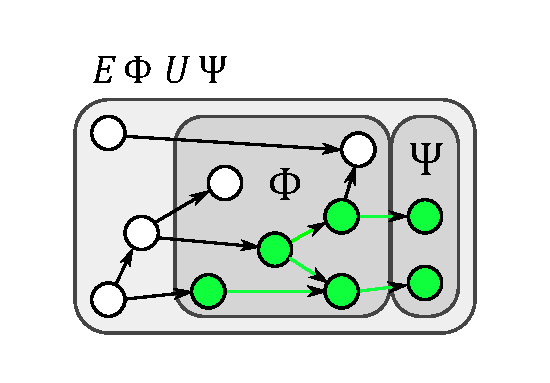
\includegraphics[width=\textwidth]{picture/Graphen/eu_zub.eps}
    \label{fig:eu_zub}  
    }
  \end{minipage}
  \begin{minipage}[b]{7 cm}
   \subfigure[ ]
   {
    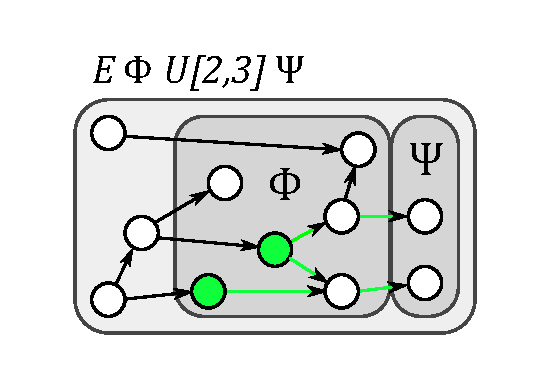
\includegraphics[width=\textwidth]{picture/Graphen/eu_zb.eps}
    \label{fig:eu_zb}
    }
  \end{minipage}
  \caption[Zustandsgraph mit Ergebnismenge einer $E \: \Phi \: U \: \Psi $ - Operation]{Beispielhafter Zustandsgraph f�r die  $E \: \Phi \: U \: \Psi $ - Operation mit Fallunterscheidung in Zeitunbeschr�nkung \ref{fig:eu_zub} und Zeitbeschr�nkung \ref{fig:eu_zb} }
  \label{fig:eu_z}
\end{figure}


...
